\documentclass[preview]{standalone}
\usepackage{tikz}

\begin{document}
  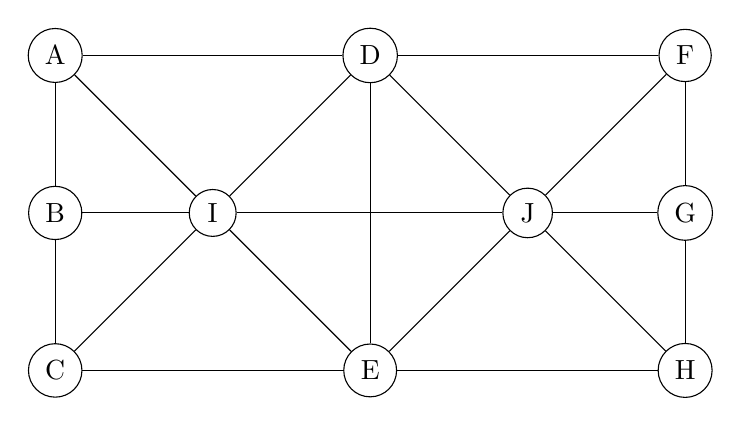
\begin{tikzpicture}
    \draw 
    (1, 1) node[circle, black, draw](C){C}
    (1, 3) node[circle, black, draw](B){B}
    (1, 5) node[circle, black, draw](A){A}
    (3, 3) node[circle, black, draw](I){I}
    (5, 1) node[circle, black, draw](E){E}
    (5, 5) node[circle, black, draw](D){D}
    (7, 3) node[circle, black, draw](J){J}
    (9, 1) node[circle, black, draw](H){H}
    (9, 3) node[circle, black, draw](G){G}
    (9, 5) node[circle, black, draw](F){F};

    \draw[-] (A) -- (B);
    \draw[-] (A) -- (I);
    \draw[-] (A) -- (D);
    \draw[-] (B) -- (I);
    \draw[-] (B) -- (C);
    \draw[-] (C) -- (I);
    \draw[-] (C) -- (E);
    \draw[-] (I) -- (D);
    \draw[-] (I) -- (E);
    \draw[-] (I) -- (J);
    \draw[-] (D) -- (E);
    \draw[-] (D) -- (J);
    \draw[-] (D) -- (F);
    \draw[-] (E) -- (J);
    \draw[-] (E) -- (H);
    \draw[-] (J) -- (F);
    \draw[-] (J) -- (G);
    \draw[-] (J) -- (H);
    \draw[-] (F) -- (G);
    \draw[-] (G) -- (H);

  \end{tikzpicture}
\end{document}
